% (c) Gerard Baecker
\documentclass[fleqn,a4paper,12pt]{article}
  \usepackage[german]{babel}
  \usepackage[utf8]{inputenc}
  \usepackage{amsmath}    % Mathematische Symbole
  \usepackage{amssymb}     % Nochmehr mathematische Symbole
  \usepackage{dsfont}      % Schriftsatz fuer Zahlenmengensymbole
  %\usepackage{verbatim}   % erweiterte Verbatim-Umgebung
  \usepackage{alltt}       % Quasi-Verbatim-Umgebung
  \usepackage{fancyhdr}    % Eigene Kopfzeilen
  \usepackage{graphicx}    % Zum Einbinden von Grafiken
  % Einbinden einer eps-Grafik geht so: includegraphics{path}
  
  % Seitenraender
  \addtolength{\voffset}{-2cm}
  \addtolength{\textheight}{0cm}
  \addtolength{\hoffset}{0cm}
  \addtolength{\textwidth}{2cm}
  \addtolength{\headheight}{2cm} % fuer jeden Strichkode einen Zentimeter
  
  % Skalierung der Grafiken
  \setlength{\unitlength}{1cm}
  
  \pagestyle{fancy}            % Eigene Kopfzeilen verwenden
  \frenchspacing               % Kein Extrafreiraum nach Satzzeichen
  \setlength{\parindent}{0pt}  % Neue Absaetze nicht einruecken
  %\sloppy                     % Schlampige Absatzformatierung
  \fussy                       % Penible Absatzformatierung
  \linespread{1.5}             % Zeilenabstand
  
  % Font fuer Code 39
  \font\xlix=wlc39 scaled 1200
  \newcommand\barcode[1]{{\xlix@#1@}}
  
  % Name, Matrikelnummer, Barcode
  \newcommand\student[2]{
    \mbox{\scriptsize
    \begin{tabular}{@{}l@{}r@{}}
      \multicolumn{2}{@{}r@{}}{\barcode{#2}}\\
      #1&#2\\
    \end{tabular}}}
  
  % Kopfzeile
  \lhead{
    \small
    \textsc{Grundlagen der Signalverarbeitung \\
      WS 2017/2018 \\
      \"Ubung (\today)}
    \vfill}
  \rhead{
    \begin{tabular}[b]{@{}rr@{}}
      \student{Philipp Badenhoop}{572693} &
      \student{Steven Lange}{568733} \\
      \student{Pascal Jochmann}{575056} &
      \student{Kevin Trogant}{572451}
    \end{tabular}}
  
  \begin{document}
  "Ubungsaufgabe 3: \newline
  Messreihe 1000 Würfe mit einem 6-seitigen Würfel: \newline
  5, 4, 2, 4, 5, 6, 3, 2, 5, 3, 4, 2, 1, 1, 5, 1, 1, 2, 1, 6, 4, 6, 1, 4, 5, 3, 2, 3, 2, 1, 1, 2, 6, 2, 5, 2, 5, 6, 4, 6, 4, 5, 2, 2, 3, 1, 2, 5, 5, 4, 5, 5, 4, 5, 2, 2, 5, 4, 3, 5, 5, 4, 2, 4, 3, 1, 5, 4, 1, 6, 5, 4, 5, 4, 2, 1, 4, 1, 2, 6, 1, 1, 5, 3, 5, 3, 1, 6, 4, 6, 1, 6, 2, 5, 4, 4, 2, 6, 1, 3, 4, 2, 2, 5, 3, 3, 2, 5, 6, 2, 3, 3, 3, 6, 3, 1, 4, 2, 1, 5, 6, 6, 3, 2, 3, 3, 5, 6, 3, 1, 4, 5, 6, 3, 1, 1, 4, 3, 1, 2, 3, 6, 3, 2, 3, 4, 2, 4, 6, 4, 3, 4, 3, 2, 4, 5, 5, 4, 3, 3, 2, 4, 4, 5, 5, 6, 4, 2, 6, 6, 5, 5, 6, 6, 2, 3, 1, 2, 3, 2, 5, 1, 3, 3, 2, 4, 5, 2, 4, 5, 3, 6, 5, 3, 5, 5, 2, 6, 4, 3, 6, 5, 5, 2, 1, 5, 5, 2, 1, 3, 2, 5, 3, 2, 2, 6, 3, 5, 4, 3, 1, 1, 5, 6, 5, 6, 3, 2, 3, 1, 6, 6, 3, 5, 3, 2, 5, 3, 2, 5, 2, 5, 3, 5, 2, 2, 1, 5, 4, 3, 6, 6, 2, 6, 3, 2, 3, 2, 4, 5, 4, 6, 3, 1, 3, 1, 3, 4, 1, 1, 1, 6, 2, 1, 5, 4, 5, 6, 2, 4, 1, 4, 2, 6, 3, 6, 1, 2, 2, 2, 3, 5, 3, 6, 2, 5, 2, 6, 5, 1, 2, 2, 5, 4, 2, 5, 6, 3, 1, 3, 1, 3, 6, 5, 3, 5, 2, 6, 4, 3, 4, 2, 2, 6, 6, 1, 2, 1, 4, 5, 1, 3, 3, 1, 6, 5, 4, 2, 1, 5, 4, 6, 6, 1, 2, 4, 1, 4, 3, 2, 2, 1, 3, 4, 3, 6, 2, 1, 4, 3, 6, 2, 1, 2, 5, 2, 6, 1, 2, 3, 1, 4, 3, 5, 6, 1, 6, 5, 2, 4, 4, 4, 2, 1, 3, 3, 3, 3, 1, 3, 6, 6, 2, 4, 1, 2, 5, 2, 6, 1, 6, 3, 2, 1, 5, 4, 3, 4, 3, 1, 6, 2, 4, 1, 5, 2, 5, 3, 4, 6, 3, 2, 6, 3, 4, 6, 1, 5, 2, 5, 5, 5, 6, 5, 2, 5, 1, 4, 2, 3, 2, 5, 5, 6, 1, 1, 2, 4, 6, 3, 4, 5, 4, 4, 1, 4, 4, 1, 2, 6, 6, 6, 1, 4, 3, 3, 5, 6, 5, 2, 3, 4, 4, 6, 5, 1, 4, 3, 3, 1, 4, 4, 4, 4, 6, 6, 1, 4, 4, 1, 1, 3, 3, 4, 4, 4, 4, 4, 1, 3, 3, 4, 3, 3, 3, 5, 6, 1, 1, 1, 2, 6, 3, 1, 5, 5, 1, 5, 5, 3, 3, 5, 6, 2, 6, 2, 3, 1, 4, 6, 4, 2, 2, 5, 5, 2, 6, 5, 5, 5, 1, 4, 4, 4, 4, 5, 5, 5, 6, 6, 4, 6, 1, 2, 6, 6, 2, 5, 1, 6, 1, 3, 1, 1, 2, 3, 1, 1, 1, 1, 1, 2, 4, 6, 3, 4, 6, 6, 3, 4, 5, 4, 4, 2, 3, 2, 4, 1, 2, 3, 5, 3, 6, 3, 6, 4, 4, 6, 3, 5, 4, 1, 4, 5, 3, 3, 5, 4, 2, 6, 4, 4, 1, 4, 1, 1, 4, 4, 6, 3, 6, 3, 2, 4, 6, 1, 3, 6, 6, 6, 3, 1, 5, 6, 6, 3, 6, 6, 5, 1, 3, 6, 1, 6, 2, 5, 4, 6, 1, 5, 5, 3, 4, 4, 6, 4, 1, 2, 6, 5, 6, 3, 6, 2, 1, 1, 2, 3, 4, 5, 4, 3, 6, 5, 6, 5, 4, 4, 1, 6, 6, 2, 1, 6, 1, 5, 2, 3, 6, 4, 1, 5, 5, 2, 2, 2, 3, 3, 4, 6, 2, 4, 2, 1, 2, 6, 1, 3, 3, 1, 6, 4, 1, 4, 6, 3, 2, 1, 4, 2, 2, 1, 1, 1, 2, 4, 5, 1, 5, 5, 4, 5, 6, 3, 1, 5, 1, 1, 5, 4, 2, 2, 2, 5, 3, 6, 6, 3, 5, 4, 4, 1, 2, 4, 5, 6, 4, 5, 1, 6, 2, 2, 2, 5, 5, 2, 3, 6, 5, 6, 6, 2, 2, 1, 1, 5, 6, 4, 3, 2, 2, 3, 2, 5, 1, 1, 2, 5, 1, 4, 6, 2, 1, 2, 2, 4, 4, 1, 6, 2, 6, 3, 5, 3, 1, 3, 5, 2, 4, 6, 3, 5, 5, 2, 1, 3, 3, 5, 3, 4, 5, 1, 2, 2, 2, 6, 6, 1, 2, 6, 1, 1, 3, 2, 3, 2, 1, 6, 2, 6, 5, 6, 3, 1, 5, 3, 2, 6, 5, 6, 4, 3, 1, 1, 1, 3, 4, 2, 3, 4, 1, 5, 4, 3, 1, 5, 6, 4, 3, 6, 5, 2, 1, 2, 5, 2, 1, 2, 2, 2, 2, 5, 4, 2, 2, 3, 3, 5, 4, 3, 2, 3, 1, 4, 4, 6, 3, 5, 1, 1, 2, 6, 3, 2, 4, 5, 1, 5, 4, 5, 5, 4, 1, 1, 5, 6, 6, 5, 6, 5, 5, 2, 5, 1, 1, 1, 2, 5, 5, 5, 1, 5, 6, 2, 4, 5, 5, 6, 6, 6, 3, 2, 2, 4, 2, 5, 5, 4, 4, 5, 4, 2, 5, 1, 1, 6, 1, 4, 6, 6, 1, 4, 6, 2, 4, 5, 6, 3, 6, 3, 4, 2, 4, 4, 2, 6, 5, 5, 1, 2, 5, 6, 1, 5, 3, 2, 5, 3, 6, 2, 2, 4, 1, 4, 4, 5, 4, 3, 1, 6 \newline
  \textbf{Häufigkeiten:}
  \begin{center}
    \begin{tabular}{ | l | l | l | }
      \hline
      Augenzahl & Anzahl der Würfe & relative Häufigkeit \\ \hline
      1 & 164 & 0.164 \\ \hline
      2 & 177 & 0.177 \\ \hline
      3 & 158 & 0.158 \\ \hline
      4 & 164 & 0.164 \\ \hline
      5 & 175 & 0.175 \\ \hline
      6 & 162 & 0.162 \\ \hline
    \end{tabular}  
  \end{center}
  \textbf{Berechnung des Medians:} \newline
  $0.164 + 0.177 + 0.158 = 0.499 \leq 0.5$ \newline
  $0.164 + 0.177 + 0.158 + 0.164 = 0.663 > 0.5$ \newline
  Der Median ist also 3 (der dritte Summand stellt Augenzahl 3 da). \newline
  \textbf{Modalwert:} \newline
  $0.177 > 0.175 > 0.164 > 0.162 > 0.158$ \newline
  Der Modalwert ist also 2. \newline
  \textbf{Mittwelwert:} \newline 
  $m_1 = \sum_{i=0}^{n-1} x_i p_i$ \newline
  $m_1 = 1*0.164 + 2*0.177 + 3*0.158 + 4*0.164 + 5*0.175 + 6*0.162 \approx 3.5$ \newline
  \textbf{Standardabweichung:} \newline
  $s = \sqrt{\sum_{i=0}^{n-1} (x_i-m_1)^2 p_i}$ \newline
  $s = \sqrt{(1-3.495)^2*0.164 + (2-3.495)^2*0.177 + (3-3.495)^2*0.158} \\\overline{+ (4-3.495)^2*0.164 + (5-3.495)^2*0.175 + (6-3.495)^2*0.162} \approx 1.7$ \newpage
  \begin{figure}
    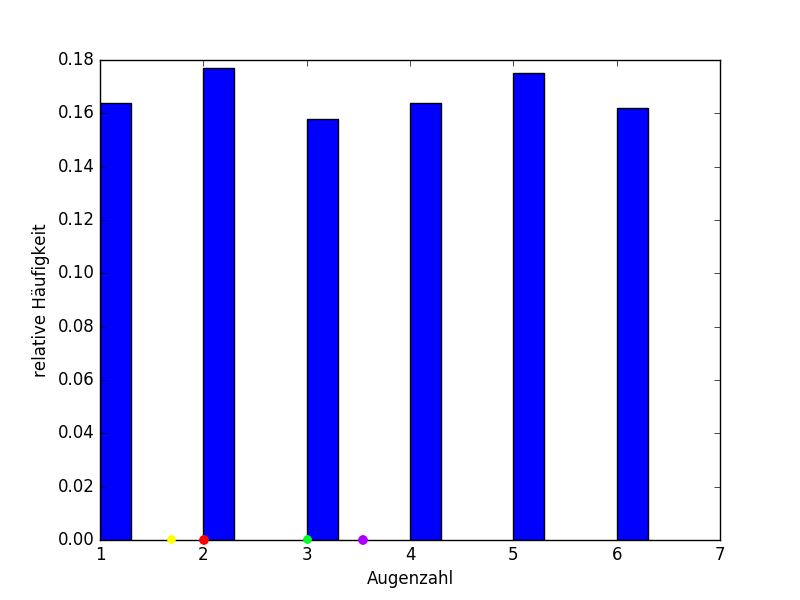
\includegraphics[width=1.0\textwidth]{histo2.png}
    \caption{Histogramm für 1000 Würfe mit einem 6-seitigen Würfel. \newline gelb: Standardabweichung, rot: Modalwert, grün: Median, violett: Mittwelwert}
  \end{figure}
  \textbf{Entropie:} \newline
  $H = \sum_{i=0}^{n-1} p_i log_2(\frac{1}{p_i})$ \newline
  $H = 0.164*log_2(\frac{1}{0.164}) + 0.177*log_2(\frac{1}{0.177}) + 0.158*log_2(\frac{1}{0.158}) + 0.164*log_2(\frac{1}{0.164}) + 0.175*log_2(\frac{1}{0.175}) + 0.162*log_2(\frac{1}{0.162}) \approx 2.58373$ \newline
  \textbf{Max. Entropie:} \newline
  $H_{max} = log_2(n)$ \newline
  $H_{max} = log_2(6) \approx 2.58496$ \newline
  \textbf{Redundanz:} \newline
  $R = H_{max} - H = 2.58496 - 2.58373 \approx 0.001$ \newline
  Die Redundanz ist sehr klein. \newline \newline
  Übungsaufgabe 4: \newline
  Messreihe Summe der Augenzahlen bei 1000 Würfe mit zwei Würfeln: \newline
  9, 9, 9, 7, 7, 6, 5, 8, 7, 8, 10, 8, 7, 2, 4, 11, 6, 7, 7, 4, 6, 8, 7, 6, 12, 6, 4, 5, 7, 3, 5, 8, 6, 8, 7, 6, 6, 9, 3, 8, 7, 6, 6, 10, 11, 12, 4, 7, 7, 8, 9, 4, 5, 10, 3, 11, 8, 8, 7, 9, 8, 7, 11, 2, 8, 5, 8, 6, 9, 11, 8, 9, 11, 8, 6, 8, 5, 8, 5, 11, 4, 7, 7, 3, 3, 10, 10, 7, 8, 5, 8, 6, 8, 3, 12, 5, 7, 4, 5, 9, 8, 6, 7, 11, 7, 7, 3, 9, 12, 5, 9, 6, 5, 8, 3, 10, 7, 11, 7, 4, 11, 3, 9, 4, 7,10, 2, 11, 4, 5, 10, 7, 3, 7, 7, 10, 11, 7, 4, 7, 3, 9, 6, 7, 8, 6, 7, 6, 8, 7, 10, 6, 4, 8, 9, 6, 7, 11, 11, 9, 8, 6, 6, 11, 9, 9, 4, 8, 5, 4, 4, 4, 7, 7, 8, 10, 5, 7, 9, 9, 7, 5, 8, 5, 8, 8, 3, 7, 5, 7, 4, 7, 8, 8, 5, 6, 4, 5, 10, 9, 4, 5, 3, 6, 5, 7, 7, 11, 5, 7, 8, 8, 5, 5, 6, 7, 6, 6, 7, 5, 9, 11, 8, 6, 6, 11, 8, 5, 8, 6, 3, 5, 3, 3, 10, 11, 8, 5, 12, 9, 11, 7, 10, 9, 7, 6, 11, 9, 7, 3, 8, 7, 2, 6, 6, 7, 4, 10, 5, 8, 7, 6, 4, 6, 9, 4, 9, 6, 10, 4, 5, 10, 11, 8, 4, 6, 10, 5, 3, 7, 8, 2, 8, 9, 6, 5, 11, 6, 5, 11, 7, 8, 6, 12, 6, 6, 10, 4, 6, 9, 10, 6, 4, 7, 7, 8, 10, 10, 4, 3, 9, 9, 9, 3, 12, 4, 12, 8, 9, 12, 10, 11, 3, 8, 8, 5, 6, 8, 10, 7, 3, 11, 5, 7, 8, 5, 5, 6, 6, 7, 7, 10, 6, 8, 4, 4, 8, 12, 5, 7, 5, 6, 4, 7, 3, 9, 3, 11, 7, 8, 4, 7, 7, 4, 5, 9, 8, 8, 2, 6, 5, 4, 6, 5, 5,8, 9, 8, 11, 5, 9, 5, 8, 6, 8, 7, 3, 8, 7, 6, 6, 7, 4, 8, 7, 8, 10, 5, 5, 7, 8, 6, 4, 6, 8, 6, 6, 9, 7, 9, 5, 11, 10, 5, 7, 9, 8, 6, 12, 6, 10, 9, 3, 4, 5, 7, 7, 7, 4, 5, 7, 3, 9, 6, 6, 8, 11, 7, 8, 7, 7, 4, 2, 9, 5, 4, 6, 5, 4, 6, 4, 5, 5, 8, 11, 4, 9, 4, 5, 9, 8, 7, 6, 12, 8, 6, 9, 3, 8, 7, 6, 5, 7, 8, 5, 6, 7, 9, 5, 5, 11, 6, 5, 8, 8, 4, 4, 9, 6, 7, 8, 12, 8, 8, 8, 5, 7, 7, 7, 12, 5, 6, 10, 12, 9, 2, 5, 8, 6, 4, 4, 4, 6, 9, 8, 2, 4, 6, 8, 8, 2, 9, 9, 8, 7, 3, 5, 9, 6, 7, 10, 9, 9, 6, 3, 8, 8, 6, 6, 10, 6, 6, 7, 5, 7, 8, 10, 7, 7, 11, 9, 10, 8, 10, 9, 9, 6, 3, 4, 6, 5, 7, 10, 3, 6, 7,8, 3, 10, 7, 11, 7, 9, 10, 8, 9, 5, 6, 9, 8, 8, 6, 5, 9, 6, 2, 4, 11, 5, 11, 10, 7, 6, 6, 10, 4, 6, 6, 3, 5, 12, 4, 4, 11, 2, 8, 9, 7, 8, 9, 8, 7, 6, 3, 8, 9, 8, 9, 8, 7, 4, 10, 6, 4, 5, 6, 5, 7, 5, 6, 8, 10, 5, 3, 8, 11, 4, 6, 7, 7, 2, 8, 8, 10, 7, 4, 11, 6, 4, 5, 4, 10, 5, 8, 7, 7, 4, 6, 7, 6, 7, 8, 6, 6, 3, 9, 4, 3, 7, 10, 12, 10, 5, 6, 8, 9, 9, 7, 4, 5, 9, 8, 3, 9, 7, 3, 6, 6, 6, 6, 8, 7,2, 12, 6, 5, 7, 8, 8, 10, 7, 5, 6, 8, 5, 3, 10, 7, 6, 8, 11, 9, 10, 8, 7, 3, 6, 8, 4, 6, 6, 3, 4, 11, 3, 10, 6, 3, 3, 12, 9, 7, 5, 7, 3, 6, 8, 5, 3, 5, 7, 9, 2, 5, 10, 8, 8, 10, 9, 12, 5, 8, 7, 7, 9, 5, 9, 10, 12, 7, 8, 4, 10, 12, 3, 7, 9, 4, 5, 12, 10, 7, 9, 12, 9, 5, 10, 2, 9, 6, 9, 4, 5, 5, 9, 7, 5, 4, 9, 7, 5, 11, 6, 4, 11, 6, 7, 7, 8, 6, 7, 4, 6, 11, 4, 5, 8, 4, 5, 7, 4, 4, 7, 7, 2, 2, 7, 11, 9, 6, 5, 6, 6, 6, 9, 7, 4, 8, 6, 4, 10, 7, 6, 6, 4, 3, 6, 5, 9, 8, 2, 9, 8, 2, 5, 6, 7, 9, 4, 3, 3, 5, 3, 4, 2, 7, 4, 2, 9, 6, 5, 5, 7, 4, 5, 10, 2, 8, 5, 5, 8, 6, 4, 8, 4, 7, 6, 7, 7, 5, 4, 2, 10, 8, 7, 4, 7, 8, 8, 9, 7, 8, 3, 4, 10, 2, 8, 12, 6, 11, 10, 7, 9, 7, 4, 6, 12, 3, 6, 7, 7, 3, 9, 6, 6, 6, 10, 6, 5, 6, 4, 3, 6, 5, 7, 5, 4, 4, 6, 8, 9, 10, 10, 7, 10, 5, 6, 12, 5, 5, 7, 9, 9, 7,11, 6, 8, 6, 7, 7, 6, 6, 12, 10, 12, 7, 6, 4, 4, 3, 8, 6, 11, 4, 2, 4, 7, 10, 10, 5, 7, 5, 9, 11, 8, 3, 12, 5, 8, 6, 7, 6, 7, 8, 9, 11, 5, 4, 6, 8, 5, 6, 6, 6, 10, 7, 12, 7, 9, 7 \newline
  \textbf{Häufigkeiten}
  \begin{center}
    \begin{tabular}{ | l | l | l | }
      \hline
      Summe der Augenzahlen & Anzahl der Würfe & relative Häufigkeit \\ \hline
      2 & 26 & 0.026 \\ \hline
      3 & 59 & 0.059 \\ \hline
      4 & 97 & 0.097 \\ \hline
      5 & 118 & 0.118 \\ \hline
      6 & 153 & 0.153 \\ \hline
      7 & 162 & 0.162 \\ \hline
      8 & 138 & 0.138 \\ \hline
      9 & 98 & 0.098 \\ \hline
      10 & 68 & 0.068 \\ \hline
      11 & 50 & 0.05 \\ \hline
      12 & 31 & 0.031 \\ \hline
    \end{tabular}  
  \end{center}
  \textbf{Median:} 7 \newline
  \textbf{Modalwert:} 7 \newline
  \textbf{Mittwelwert:} 6.847 \newline
  \textbf{Standardabweichung:} $\approx 2.4$ \newline
  \textbf{Entropie:} $\approx 3.2658$ \newline
  \textbf{Max. Entropie:} $\approx 3.4594$ \newline
  \textbf{Redundanz:} $\approx 0.194$ \newline
  \begin{figure}
    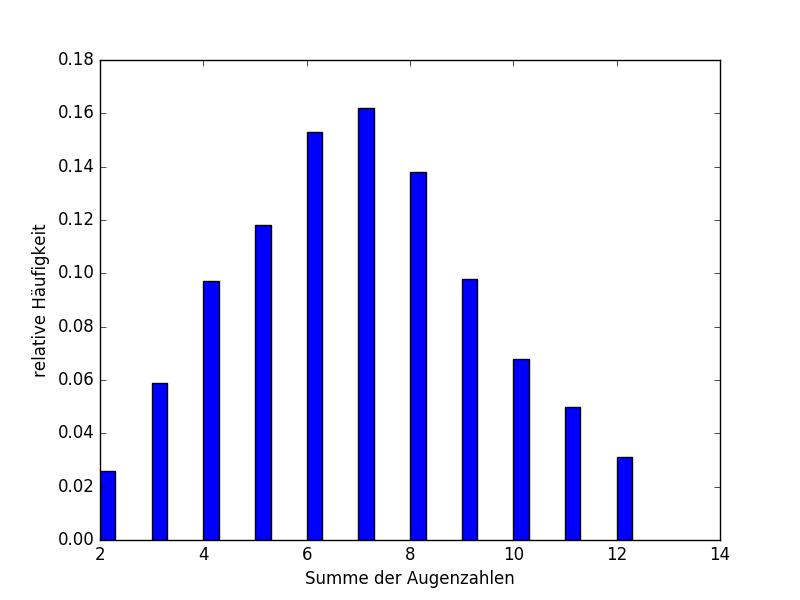
\includegraphics[width=1.0\textwidth]{histo3.png}
    \caption{Normales Histogramm für die Summe der Augenzahlen mit zwei Würfeln bei 1000 Würfen}
  \end{figure}
  \begin{figure}
    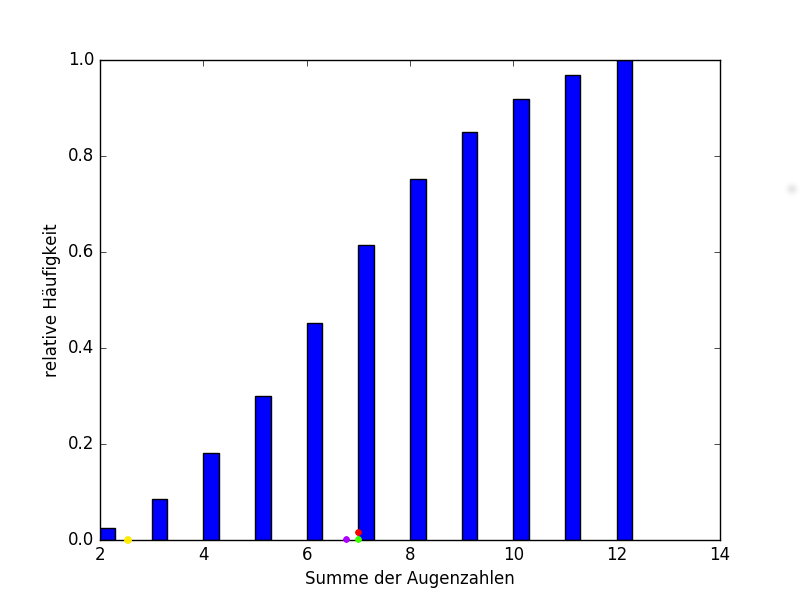
\includegraphics[width=1.0\textwidth]{histo5.png}
    \caption{Kumulative Histogramm für die Summe der Augenzahlen mit zwei Würfeln bei 1000 Würfen \newline gelb: Standardabweichung, rot: Modalwert, grün: Median, violett: Mittwelwert}
  \end{figure}
  \newpage
  \newpage
	Übungsaufgabe 6: \newline
	Das Histogramm beschreibt eine Wahrscheinlichkeitsdichtefunktion. Die Fl\"ache unter der Funktion $p(x)$ ist gleich 1. \\
	Der Mittelwert ist $m = \frac{a+b}{2} = \frac{7}{2} = 3,5$ \\
	Der Varianz ist $v = \frac{(b-a)^2}{12} = \frac{36}{12} = 3 $ \\
  Die Standardabweichung ist $\sqrt{v} = 1,732$
  \begin{figure}
		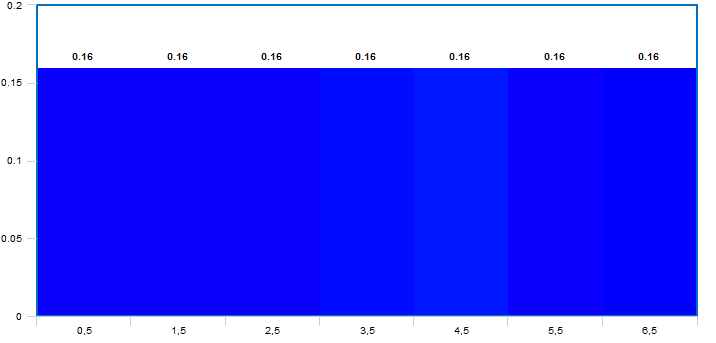
\includegraphics[width=1.0\textwidth]{H1.PNG}
		\caption{normiertes Histogramm f\"ur runden W\"urfel}
	\end{figure}
  \end{document}

  
